%%%%%%%%%%%%%%%%%%%%%%%%%%%%%%%%%%%%%%%%%%%%%%%%%%%%%%%%%%%%%%%%%%%%%%%%%%%%%%%
%% Chapter: Causal Bandits and Adaptive Experimentation
%% Section label: section:adaptive_experiments
%%
%% Split from ch10b_rl_for_ci/tex/rl_for_ci.tex on 2026-07-23 along the
%% offline-estimation vs adaptive-design seam. This chapter owns the design
%% side: causal bandits (MABUC, Lattimore) and adaptive experimentation with
%% post-experiment inference (Kasy-Sautmann, Hadad, Bibaut), plus the
%% causal-bandit simulation. The estimation side (DTR bridge, OPE, dynamic
%% DML, offline policy learning) stays in ch10b_rl_for_ci.
%%%%%%%%%%%%%%%%%%%%%%%%%%%%%%%%%%%%%%%%%%%%%%%%%%%%%%%%%%%%%%%%%%%%%%%%%%%%%%%

%%%%%%%%%%%%%%%%%%%%%%%%%%%%%%%%%%%%%%%%%%%%%%%%%%%%%%%%%%%%%%%%%%%%%%%%%%%%%%%
%% Chapter intro
%%%%%%%%%%%%%%%%%%%%%%%%%%%%%%%%%%%%%%%%%%%%%%%%%%%%%%%%%%%%%%%%%%%%%%%%%%%%%%%

The preceding chapter estimated the value and the structural parameters of dynamic policies from data that had already been collected. This chapter turns to the collection itself, asking how sequential-decision algorithms should gather the data from which causal conclusions will be drawn. In a standard multi-armed bandit the learner treats each arm as an opaque black box, accumulating reward observations until it can distinguish the best arm from the rest. When the reward-generating mechanism is described by a known causal graph, the learner can exploit that structure to propagate information across arms. \citet{bareinboim2015mabuc} showed that standard bandit algorithms incur linear cumulative regret on environments with unobserved confounders, because the observational and interventional distributions can both be uninformative, and introduced causal Thompson sampling to exploit counterfactual contrasts. \citet{lattimore2016causal} formalized the gain from graph knowledge as a regret bound that depends on a graph-derived hardness parameter rather than the number of arms, yielding strict improvement whenever the arm distribution has at least one extreme coordinate.

This chapter develops two threads in turn. The first covers causal bandits, examining both the confounding-corrected exploration of \citet{bareinboim2015mabuc} and the graph-aware exploration of \citet{lattimore2016causal}. The second covers the adaptive-experimentation literature, where the design problem and the inference problem must be solved jointly over a multi-wave sequential trial, combining bandit assignment with valid post-experiment inference. The estimation toolkit that these designs feed, off-policy evaluation and dynamic treatment effect inference under sequential ignorability, is developed in Chapter~\ref{section:rl_for_ci}.

%%%%%%%%%%%%%%%%%%%%%%%%%%%%%%%%%%%%%%%%%%%%%%%%%%%%%%%%%%%%%%%%%%%%%%%%%%%%%%%
\subsection{Causal Bandits}
\label{subsec:causal_bandits}
%%%%%%%%%%%%%%%%%%%%%%%%%%%%%%%%%%%%%%%%%%%%%%%%%%%%%%%%%%%%%%%%%%%%%%%%%%%%%%%

The multi-stage problems of Chapter~\ref{section:rl_for_ci} let the state evolve under the influence of past treatments. This subsection collapses the horizon to a single stage but expands the structure of the action set, replacing the opaque arms of a standard multi-armed bandit with interventions on a known causal graph. The resulting "causal bandit" setting was introduced by \citet{bareinboim2015mabuc} for the case of unobserved confounders between the agent's choice and the reward, and formalized into a regret theorem by \citet{lattimore2016causal}.

\subsubsection*{Bandits under unobserved confounding}

The motivating example of \citet{bareinboim2015mabuc} is a "greedy casino" with two slot machines $M_1$ and $M_2$. An unobserved binary variable $D$ (the player is drunk) and an unobserved binary variable $B$ (the chosen machine is blinking) jointly determine the gambler's natural arm choice $X \in \{M_1, M_2\}$ via a structural equation $X = f(D, B)$. Both confounders also affect the reward $Y$. The casino parameters are chosen so that the observational distribution and the interventional distribution are both flat,
\begin{equation}
\mathbb{P}(Y = 1 \mid X = M_j) = \mathbb{P}(Y = 1 \mid \mathrm{do}(X = M_j)) = \tfrac{1}{2}, \qquad j \in \{1, 2\}.
\label{eq:mabuc_degenerate}
\end{equation}
\citet{bareinboim2015mabuc} run $\epsilon$-greedy, UCB1, Thompson Sampling, and EXP3 on this environment and observe that all four are statistically indistinguishable from random guessing, with linear cumulative regret. The reason is that both the observational and interventional distributions average out the contribution of the confounders, leaving no signal at all in the average payoff per arm.

The fix proposed in \citet{bareinboim2015mabuc} is to refine the decision objective from the marginal interventional value to the \emph{effect of treatment on the treated}, that is, to condition on the agent's own natural intuition $X = x$ and ask what the payoff would have been under an alternative action,
\begin{equation}
a^* = \arg\max_{a}\, \mathbb{E}\!\left[Y_{X = a} = 1 \,\big|\, X = x\right].
\label{eq:rdc}
\end{equation}
The authors call this the \emph{Regret Decision Criterion}. Equation~\eqref{eq:rdc} is generally not identified from observational and interventional data alone, but in the binary case it can be recovered through algebraic combinations of $\mathbb{P}(Y \mid X)$ and $\mathbb{P}(Y \mid \mathrm{do}(X))$, and in the general case through intention-specific randomization that interrupts the agent before action selection. Plugging this counterfactual quantity into Thompson Sampling yields Causal Thompson Sampling ($\text{TS}_C$), which seeds Beta posteriors from observational data via the consistency axiom and biases sampling via the relative-difference-of-confounders (RDC) weighting that suppresses arms whose interventional value varies sharply across contexts. In the greedy casino, $\text{TS}_C$ achieves bounded cumulative regret while standard Thompson Sampling grows linearly. The simulation in Section~\ref{subsec:causal_bandit_sim} implements both the full $\text{TS}_C$ of \citet{bareinboim2015mabuc} (Algorithm~1, with consistency-axiom seeding of the off-intuition arm at fractional pseudo-count $c = 0.5$ and RDC weighting $w_a = \mathrm{clip}(1 - |\hat Q_1(a) - \hat Q_2(a)|, 0.01, 1)$ on running cell means $\hat Q_x(a)$) and a minimal context-conditional Thompson sampling (CCTS) baseline that retains only the $(x, a)$ posterior without seeding or weighting. The two-algorithm comparison lets the reader isolate the contribution of the additional Bareinboim components on this specific MDP.

\subsubsection*{Causal-graph-aware exploration}

\citet{lattimore2016causal} formalize the gain from exploiting causal structure as a regret theorem. They study the parallel-bandit special case: $N$ binary parents $X_1, \ldots, X_N$ of a binary reward $Y$, with action set $\mathcal{A} = \{\mathrm{do}()\} \cup \{\mathrm{do}(X_i = j) : i \in [N], j \in \{0,1\}\}$. After each action the learner observes both $Y$ and the realized values of all non-intervened parents. Their Algorithm~1 spends half the budget on $\mathrm{do}()$ to estimate the marginal probabilities $q_i = \mathbb{P}(X_i = 1)$ and uses the post-action observations to credit-assign across all arms. The remaining budget is allocated to the actions whose direct-observation probability is smallest, with the cutoff $\tau$ chosen to optimize the worst-case regret. Define the graph-derived hardness
\begin{equation}
m(q) = \min_{\tau \in \{2, \ldots, N\}} \max\!\left(\tau,\, \bigl|\{i : \min(q_i, 1 - q_i) < 1/\tau\}\bigr|\right) \in [2, N].
\label{eq:lattimore_m}
\end{equation}
Theorem~1 of \citet{lattimore2016causal} gives the simple-regret guarantee for Algorithm~1,
\begin{equation}
R_T(\text{Algorithm 1}) = \tilde O\!\left(\sqrt{m(q)/T}\right),
\label{eq:lattimore_regret}
\end{equation}
and Theorem~2 establishes the matching lower bound $R_T = \Omega(\sqrt{m(q)/T})$ over all algorithms. Standard best-arm-identification procedures that ignore the graph achieve $\Omega(\sqrt{N/T})$ \citep[Theorem~4]{lattimore2016causal}, so the graph-aware algorithm strictly improves whenever $m(q) < N$, equivalently, whenever the parent distribution has at least one extreme coordinate. In the balanced case $q = (\tfrac{1}{2}, \ldots, \tfrac{1}{2})$ the hardness collapses to $m(q) = 2$ regardless of $N$; in the degenerate case $q = (0, \ldots, 0)$ the graph provides no help and $m(q) = N$. For general directed acyclic graphs Algorithm~2 of \citet{lattimore2016causal} uses a truncated importance-weighted estimator with a mixing distribution $\eta$ over interventions, achieving simple regret $\tilde O(\sqrt{m(\eta)/T})$ where $m(\eta)$ is the analogous graph-derived hardness; for the parallel bandit case $m(\eta) = m(q)$.

In reinforcement-learning vocabulary, the MABUC instance is \emph{causal Thompson sampling}, in which the Beta posterior is indexed not by arm alone but by the agent's natural intuition $X = x$ that conditions the counterfactual reward distribution, and the Regret Decision Criterion is the Bayesian-bandit analog of an advantage estimate under unobserved confounding. The parallel-bandit Algorithm~1 is \emph{graph-aware UCB}, a deterministic budget split that exploits the post-action observations of non-intervened parents as additional samples for arms that were not pulled.

The simulation study in Section~\ref{subsec:causal_bandit_sim} reproduces the $\sqrt{m/T}$ rate for Algorithm~1 on the monotone segment of the hardness grid $m \in \{2, 8, 24\}$ at $N = 50$, contrasted with the asymptotic $\sqrt{N/T}$ rate lower bound for a graph-blind best-arm-identification baseline, and includes the greedy-casino instance of \citet{bareinboim2015mabuc} with both the full $\mathrm{TS}_C$ algorithm (consistency-axiom seeding plus RDC weighting) and a minimal context-conditional Thompson sampling baseline to demonstrate the value of causal reasoning under unobserved confounders.

%%%%%%%%%%%%%%%%%%%%%%%%%%%%%%%%%%%%%%%%%%%%%%%%%%%%%%%%%%%%%%%%%%%%%%%%%%%%%%%
\subsection{Adaptive Experimentation and Post-Experiment Inference}
\label{subsec:adaptive_experiments}
%%%%%%%%%%%%%%%%%%%%%%%%%%%%%%%%%%%%%%%%%%%%%%%%%%%%%%%%%%%%%%%%%%%%%%%%%%%%%%%

The causal-bandit setting of Section~\ref{subsec:causal_bandits} fixes the data-generating process and the action set and asks how to learn the best intervention. This subsection considers the dual concern. When the data themselves are collected adaptively by a Thompson-sampling-style assignment rule that the experimenter designs, what does optimal design look like, and how should the analyst conduct valid statistical inference on the resulting data? \citet{kasy2021adaptive} answer the design question; \citet{hadad2021adaptive} answer the inference question. The two papers address different parts of the same applied workflow. First design a multi-wave adaptive experiment that ends in a policy choice, then deliver confidence intervals on the welfare gain.

\subsubsection*{Design: exploration sampling for policy choice}

\citet{kasy2021adaptive} consider a finite-horizon adaptive experimental design problem with $K$ candidate treatments, $T$ waves of approximately equal size, and a welfare objective equal to the average outcome of the policy chosen at the end of the experiment. Unlike the in-sample welfare objective targeted by classical bandit algorithms, this objective values only the post-experiment policy, not the participants' realizations during the experiment. The authors prove this distinction matters. Standard Thompson sampling, which assigns each treatment $d$ at wave $t$ with probability equal to the posterior probability $p_t^d$ that $d$ is optimal given history, is not rate-optimal for policy choice, because Thompson sampling concentrates on a single top treatment fast enough to starve the suboptimal treatments of the samples needed to verify their suboptimality.

The proposed correction is \emph{exploration sampling}. Replace the Thompson assignment probability $p_t^d$ with a concave transformation that flattens at the top,
\begin{equation}
q_t^d = S_t \cdot p_t^d \cdot (1 - p_t^d),
\label{eq:exploration_sampling}
\end{equation}
where $S_t$ is a normalizing constant. Two consequences follow. First, no treatment ever receives more than 50\% of the sample at any wave, regardless of how confident the posterior becomes. Second, in large samples the assignment shares converge to a non-random vector $\rho^d$ for which the posterior probability of suboptimality decays at the same exponential rate for every suboptimal treatment; power for rejection is equalized. Theorem~1 of \citet{kasy2021adaptive} establishes that exploration sampling attains the best exponential rate of expected policy regret subject to the constraint that the top treatment receives at most half the sample, a constraint that the paper's Proposition~2 shows loses at most a factor of two relative to the fully optimal allocation.

The empirical anchor is a field experiment with Precision Agriculture for Development (PAD) in India, deploying exploration sampling across 17 waves of approximately 600 farmers each, comparing six recruitment strategies for an agricultural extension service. The realized assignment trajectory matches the theoretical prediction. The top treatment receives close to but not above half the sample, and posterior probabilities for suboptimal treatments converge to zero at comparable rates. The full experiment identifies the optimal recruitment strategy with posterior probability above 0.75 after roughly $10{,}000$ participants.

\subsubsection*{Inference: adaptively-weighted AIPW after the experiment}

Once the experiment in \citet{kasy2021adaptive} has run, the analyst still needs valid confidence intervals on the welfare of the chosen policy and on the contrasts between treatments. This is harder than it looks. \citet{hadad2021adaptive} show that the obvious estimators all fail. The sample mean of $Y_t$ within each arm is biased downward whenever a temporary downward fluctuation in the early phase of the experiment causes that arm to be sampled less in later phases. The inverse-propensity-weighted estimator $\hat Q^{\text{IPW}}(w) = T^{-1} \sum_t \mathbb 1\{W_t = w\} Y_t / e_t(w)$ is unbiased but heavy-tailed, because the inverse weights $1/e_t(w)$ grow without bound as the bandit algorithm down-weights an arm. The vanilla augmented inverse-propensity score
\begin{equation}
\hat\Gamma_t^{\text{AIPW}}(w) = \hat m_t(w) + \frac{\mathbb 1\{W_t = w\}}{e_t(w)}\bigl(Y_t - \hat m_t(w)\bigr)
\label{eq:hadad_aipw_score}
\end{equation}
inherits the same heavy-tailed behavior when averaged uniformly across time, because the conditional variances of its components depend on $1/e_t(w)$ and can diverge as the bandit assignment probabilities approach zero.

The solution proposed in \citet{hadad2021adaptive} is to non-uniformly average the AIPW scores using history-adapted evaluation weights $h_t(w)$ that compensate for the propensity decay. The \emph{adaptively-weighted AIPW estimator} is
\begin{equation}
\hat Q^{\text{AW}}(w) = \frac{\sum_{t=1}^T h_t(w)\, \hat\Gamma_t^{\text{AIPW}}(w)}{\sum_{t=1}^T h_t(w)}.
\label{eq:adaptive_aipw}
\end{equation}
Their Theorem~2 establishes that for any history-adapted weights satisfying an infinite-sampling condition, a variance-convergence condition, and a Lyapunov-type moment condition, the studentized statistic is asymptotically standard normal. The simplest choice that satisfies these conditions and approximately minimizes asymptotic variance is the constant-allocation-rate weight $h_t(w) \propto \sqrt{e_t(w)}$, which compensates for propensity decay at exactly the right rate. The empirical demonstration in their Section~4 reports near-nominal 95\% coverage of confidence intervals constructed from the studentized statistic under Thompson-sampling data collection, while the sample mean and the IPW estimator both fail.\footnote{\citet{bibaut2021post} extend the adaptively-weighted AIPW framework to contextual adaptive experiments, where the assignment rule may depend on per-unit covariates. Their CADR estimator inversely weights each canonical-gradient term by an adaptively estimated conditional standard deviation, producing the first asymptotically-normal post-bandit estimator that works with contextual bandit data. The construction requires no outcome-model consistency, only that the conditional-standard-deviation estimator be measurable with respect to past data.}

Together, \citet{kasy2021adaptive} and \citet{hadad2021adaptive} complete the adaptive-experimentation workflow. The first paper says what assignment rule maximizes the welfare of the post-experiment policy choice; the second paper says how to construct valid confidence intervals on the resulting welfare estimates. Both treat the assignment mechanism as a Thompson-family bandit, and both deliver formal optimality results: rate-optimality for the design \citep[Theorem~1]{kasy2021adaptive} and asymptotic normality for the inference \citep[Theorem~2]{hadad2021adaptive}. The use of an RL algorithm at the design stage of a field experiment, with causal-inference guarantees at the inference stage, is the cleanest example in this chapter of the RL-for-CI narrative bridging from theory to deployed practice.

In reinforcement-learning vocabulary, exploration sampling is a \emph{welfare-objective Thompson-sampling variant} that trades in-sample cumulative-regret optimality for post-experiment power equalisation across suboptimal arms. The adaptively-weighted AIPW estimator is the \emph{propensity-decay-robust off-policy-evaluation estimator} that any reinforcement-learning pipeline collecting adaptive data needs in order to recover valid inference from its own logged data, whether the adaptive collection is a contextual bandit, an online RL algorithm with an off-policy correction, or a preference-elicitation loop for RLHF.

%%%%%%%%%%%%%%%%%%%%%%%%%%%%%%%%%%%%%%%%%%%%%%%%%%%%%%%%%%%%%%%%%%%%%%%%%%%%%%%
\subsection{Simulation Study: Causal Bandits on the Parallel-Bandit Family}
\label{subsec:causal_bandit_sim}
%%%%%%%%%%%%%%%%%%%%%%%%%%%%%%%%%%%%%%%%%%%%%%%%%%%%%%%%%%%%%%%%%%%%%%%%%%%%%%%

This subsection presents the computational experiment that grounds Section~\ref{subsec:causal_bandits}. Three claims are put to the test. On the parallel-bandit family the graph-aware algorithm of \citet{lattimore2016causal} degrades monotonically in the graph hardness $m(q)$ while a graph-blind best-arm-identification baseline is flat in it, its simple regret decays at the $T^{-1/2}$ rate of Theorem~1, and on the greedy-casino instance of \citet{bareinboim2015mabuc} the counterfactual quantity that $\mathrm{TS}_C$ identifies buys a strict improvement over a context-conditional posterior that does not identify it.

Each claim is separated from the design choice that would otherwise confound it. Hardness and horizon are varied in different panels, because the $\tilde O(\sqrt{m(q)/T})$ bound of Theorem~1 is minimax over instances rather than a decay rate on any one of them, so a panel run at a fixed reward gap cannot exhibit it. The two $\mathrm{TS}_C$ components are varied in a full factorial, because a comparison of the assembled algorithm against a baseline prices the pair jointly and cannot say which one carries the result.

The data-generating process matches the parallel-bandit setting of \citet[\S3]{lattimore2016causal}. The reward $Y$ depends on $N = 50$ binary parents $X_1, \ldots, X_N$ through a single high-leverage coordinate: $\mathbb{E}[Y \mid X] = 0.5 + \epsilon$ if $X_w = 1$ and $0.5 - \epsilon$ otherwise, with $\epsilon = 0.3$ and the index $w$ drawn uniformly at random per replication. The action set has $2N + 1 = 101$ arms: the empty intervention $\mathrm{do}()$ and each binary intervention $\mathrm{do}(X_i = j)$. Under the observational distribution each parent $X_i$ is Bernoulli with mean $q_i$; the graph-derived hardness
\begin{equation}
m(q) = \min_{\tau \in \{2, \ldots, N\}}\, \max\!\left(\tau,\ \big|\{i : \min(q_i, 1 - q_i) < 1/\tau\}\big|\right) \in [2, N]
\label{eq:simB2_m}
\end{equation}
is controlled by setting exactly $m^*$ coordinates of $q$ to an extreme value $e$ and the remainder to $0.5$. A balanced coordinate never enters the set in Equation~\eqref{eq:simB2_m} for $\tau \geq 2$, and an extreme one enters it exactly when $\tau < 1/e$, so $m(q) = \min(m^*, \lceil 1/e \rceil)$. The extreme value must therefore scale with the target, $e = 1/(2m^*)$; a value fixed independently of $m^*$ saturates the hardness at $\lceil 1/e \rceil$ and silently collapses the upper cells of the grid onto a common instance.\footnote{The realized $m(q)$ is recomputed from Equation~\eqref{eq:simB2_m} for every replication and reported alongside its label, so a construction that misses its target is visible rather than assumed.}

Four algorithms are compared. \emph{Successive Reject} \citep[Audibert and Bubeck 2010, as in][]{lattimore2016causal} is the graph-blind best-arm-identification baseline that allocates the budget across all $2N + 1$ arms using the standard logarithmic schedule. \emph{Lattimore Algorithm~1} spends $T/2$ rounds on $\mathrm{do}()$ to estimate the parent propensities and the conditional means $\hat{\mathbb{P}}(Y \mid X_i = j)$ that identify each direct-causal arm in the parallel graph, then allocates the remaining $T/2$ rounds uniformly across the unbalanced arms whose direct-observation probability falls below $1/\hat\tau^*$. \emph{Context-conditional Thompson sampling} (CCTS) is the minimal causal baseline: it maintains a Beta posterior indexed by $(x, a)$, seeded along the on-intuition diagonal $a = x$ from observational data, and at each step samples from the intuition-conditional posterior with straight argmax over arms. \emph{Full $\mathrm{TS}_C$} of \citet{bareinboim2015mabuc} Algorithm~1 augments CCTS in two ways. First, it seeds the counter-intuitive cell, which no observational sample ever visits, from the \emph{effect of treatment on the untreated}. Decomposing the interventional marginal over the latent intuition and applying consistency \citep[\S 3.6]{pearl2009causality} to the term the observational log identifies gives
\begin{equation}
\mathbb{P}(y \mid \mathrm{do}(a)) = \mathbb{P}(X = a)\, \mathbb{P}(y \mid X = a) + \mathbb{P}(X \neq a)\, \mathbb{E}[Y_a \mid X \neq a],
\label{eq:simB2_ett}
\end{equation}
which solves for $\mathbb{E}[Y_a \mid X \neq a]$ in terms of two marginals the agent holds. Neither marginal equals the counterfactual: in the greedy casino they are $0.10$ and $0.30$ while Equation~\eqref{eq:simB2_ett} returns exactly $0.50$, the true payoff of defying intuition. Second, the agent weights its posterior samples by the RDC factor $w = \mathrm{clip}(1 - |Q_1 - Q_2|, 0.01, 1)$, applied to whichever arm the contrast disfavours, where $Q_1 = \mathbb{E}[Y_{X = x'} \mid X = x]$ is the payoff of defying intuition and $Q_2 = \mathbb{P}(y \mid X = x)$ the payoff of following it. Both are conditioned on the same realized intuition, so the contrast measures which way to lean in the context the agent is actually in. The vanilla Thompson sampling baseline ignores intuition entirely and tracks a single Beta posterior per arm.

The interventional marginal in Equation~\eqref{eq:simB2_ett} comes from a separate log of randomized play that records the arm and the reward but not the intuition, which is what makes the identity necessary rather than decorative. A context-conditional learner cannot file those samples under any cell, so CCTS is given the same two logs and can use only the observational one. The difference between the two algorithms is then the causal reasoning alone, not an information advantage.

The hardness panel runs two thousand replications on the grid $m^* \in \{2, 8, 24, 48\}$ at horizon $T = 400$ and gap $\epsilon = 0.3$. The horizon panel runs one thousand replications on $T \in \{400, 800, 1600, 3200, 6400\}$ at fixed hardness $m^* = 8$, with the gap shrinking as $\epsilon_T = \sqrt{m^*/T}$. Both departures from a single fixed design are forced by what the theorem says. At a fixed gap the best arm is identified outright once the budget is large, so simple regret falls faster than any power of $T$ and the panel measures the onset of certainty rather than a rate; letting the gap track $\sqrt{m^*/T}$ holds the instance on the minimax frontier where Theorem~1 is stated. Hardness is held at $m^* = 8$ rather than at the top of the grid because $m(q)/N$ approaches one there and the graph, by construction, has nothing left to buy.

For the MABUC experiment five hundred replications are run at $T = 1000$ using the greedy-casino payoffs of \citet[Table~1]{bareinboim2015mabuc}: under each of two unobserved-confounder configurations $X \in \{0, 1\}$, following the agent's natural intuition yields payoff $0.1$ and going against it yields $0.5$. The observational distribution and the experimental distribution both average out to $0.5 \times 0.1 + 0.5 \times 0.5 = 0.3$ per arm, making standard Thompson sampling unable to distinguish the arms in expectation. Both logs hold two hundred samples, and all variants share one random seed per replication so the contrasts are paired rather than independent draws.

Tables~\ref{tab:simB2}--\ref{tab:simB2_mabuc} and Figure~\ref{fig:simB2} report the results.\footnote{Simulation source: \texttt{ch10c\_adaptive\_experiments/sims/causal\_bandit\_parallel.py}.} Successive Reject is flat in $m^*$, moving from $0.282$ to $0.298$ across the grid, which is what a graph-blind procedure should do since the hardness of the graph is invisible to it. Lattimore Algorithm~1 is monotone in $m^*$ over the whole grid, at $0.000$, $0.005$, $0.117$ and $0.234$, and the realized $m(q)$ equals its label in every replication. The allocation diagnostic shows the mechanism: the share of replications in which phase~2 reaches the optimal arm rises from $0.041$ at $m^* = 2$ to $0.890$ at $m^* = 48$, tracking the probability that the high-leverage coordinate is one of the unbalanced ones. Regret divided by $\sqrt{m^*/T}$ is not constant across this panel, at $0.000$, $0.037$, $0.479$ and $0.677$, so the panel establishes the ordering in $m(q)$ and the separation from the graph-blind baseline, not the rate.

The rate is established in the horizon panel, where the gap rides the minimax frontier. Lattimore Algorithm~1 falls from $0.0591$ at $T = 400$ to $0.0162$ at $T = 6400$, a fitted log-log slope of $-0.48$ against the $-0.5$ of Theorem~1, and holds a stable factor of roughly $2.4$ over Successive Reject across the range. In the greedy casino, vanilla Thompson sampling accumulates $200.49$ at $T = 1000$, linear in $T$ as predicted, CCTS accumulates $0.69$, and $\mathrm{TS}_C$ accumulates $0.00$. The factorial locates the improvement in the counterfactual seed rather than in the pair: seeding from Equation~\eqref{eq:simB2_ett} alone reaches $0.00$, the RDC weighting alone improves CCTS to $0.30$, and the two together add nothing further because the first already attains the floor. The seeding diagnostic reports the counter-intuitive cell at posterior mean $0.427$ and $0.476$ against a true $0.50$ before the first round, so the agent begins where CCTS must spend its burn-in arriving. Sweeping the log size confirms the direction: $\mathrm{TS}_C$ improves from $1.31$ at twenty-five samples to $0.00$ at two hundred, while CCTS improves only from $2.87$ to $0.57$, since additional interventional samples are unusable by a learner that cannot attribute them to a context.

\begin{table}[htbp]
\centering
\caption{Causal bandits on the parallel-bandit family. Simple regret (mean, standard error in parentheses) for the graph-blind Successive Reject baseline and the graph-aware Lattimore Algorithm~1 across the graph-hardness grid, at horizon $T = 400$, $N = 50$ parents, gap $\epsilon = 0.3$, two thousand Monte Carlo replications per cell. The realized $m(q)$ equals its column label in every replication.}
\label{tab:simB2}
\begin{tabular}{lrrrr}
\toprule
Method  & $m = 2$ & $m = 8$ & $m = 24$ & $m = 48$ \\
\midrule
Successive Reject & 0.282 (0.002) & 0.282 (0.003) & 0.289 (0.005) & 0.298 (0.006) \\
Lattimore Alg 1 & 0.000 (0.000) & 0.005 (0.001) & 0.117 (0.004) & 0.234 (0.006) \\
\bottomrule
\end{tabular}

\end{table}

\begin{table}[htbp]
\centering
\caption{Greedy-casino MABUC, full factorial over the two $\mathrm{TS}_C$ components. Cumulative regret (mean, standard error in parentheses) at horizon $T = 1000$ over five hundred Monte Carlo replications, rank-ordered by mean regret, with all variants sharing one seed per replication. The row with an observational seed and no RDC weighting is CCTS. The consistency-copy rows substitute a seed taken from the on-intuition outcome for the one identified by Equation~\eqref{eq:simB2_ett}.}
\label{tab:simB2_mabuc}
\begin{tabular}{lrr}
\toprule
Algorithm & Regret at $T = 100$ & Regret at $T = 1000$ \\
\midrule
$\mathrm{TS}_C$: ETT seed $+$ RDC \citep{bareinboim2015mabuc} & 0.00 & 0.00 (0.00) \\
ETT seed, no RDC & 0.00 & 0.00 (0.00) \\
Observational seed $+$ RDC & 0.30 & 0.30 (0.02) \\
CCTS (observational seed, no RDC) & 0.69 & 0.69 (0.04) \\
Consistency-copy seed $+$ RDC & 0.79 & 0.79 (0.04) \\
Consistency-copy seed, no RDC & 4.47 & 4.52 (0.11) \\
Vanilla Thompson sampling & 19.98 & 200.49 (0.28) \\
\bottomrule
\end{tabular}

\end{table}

\begin{figure}[htbp]
\centering
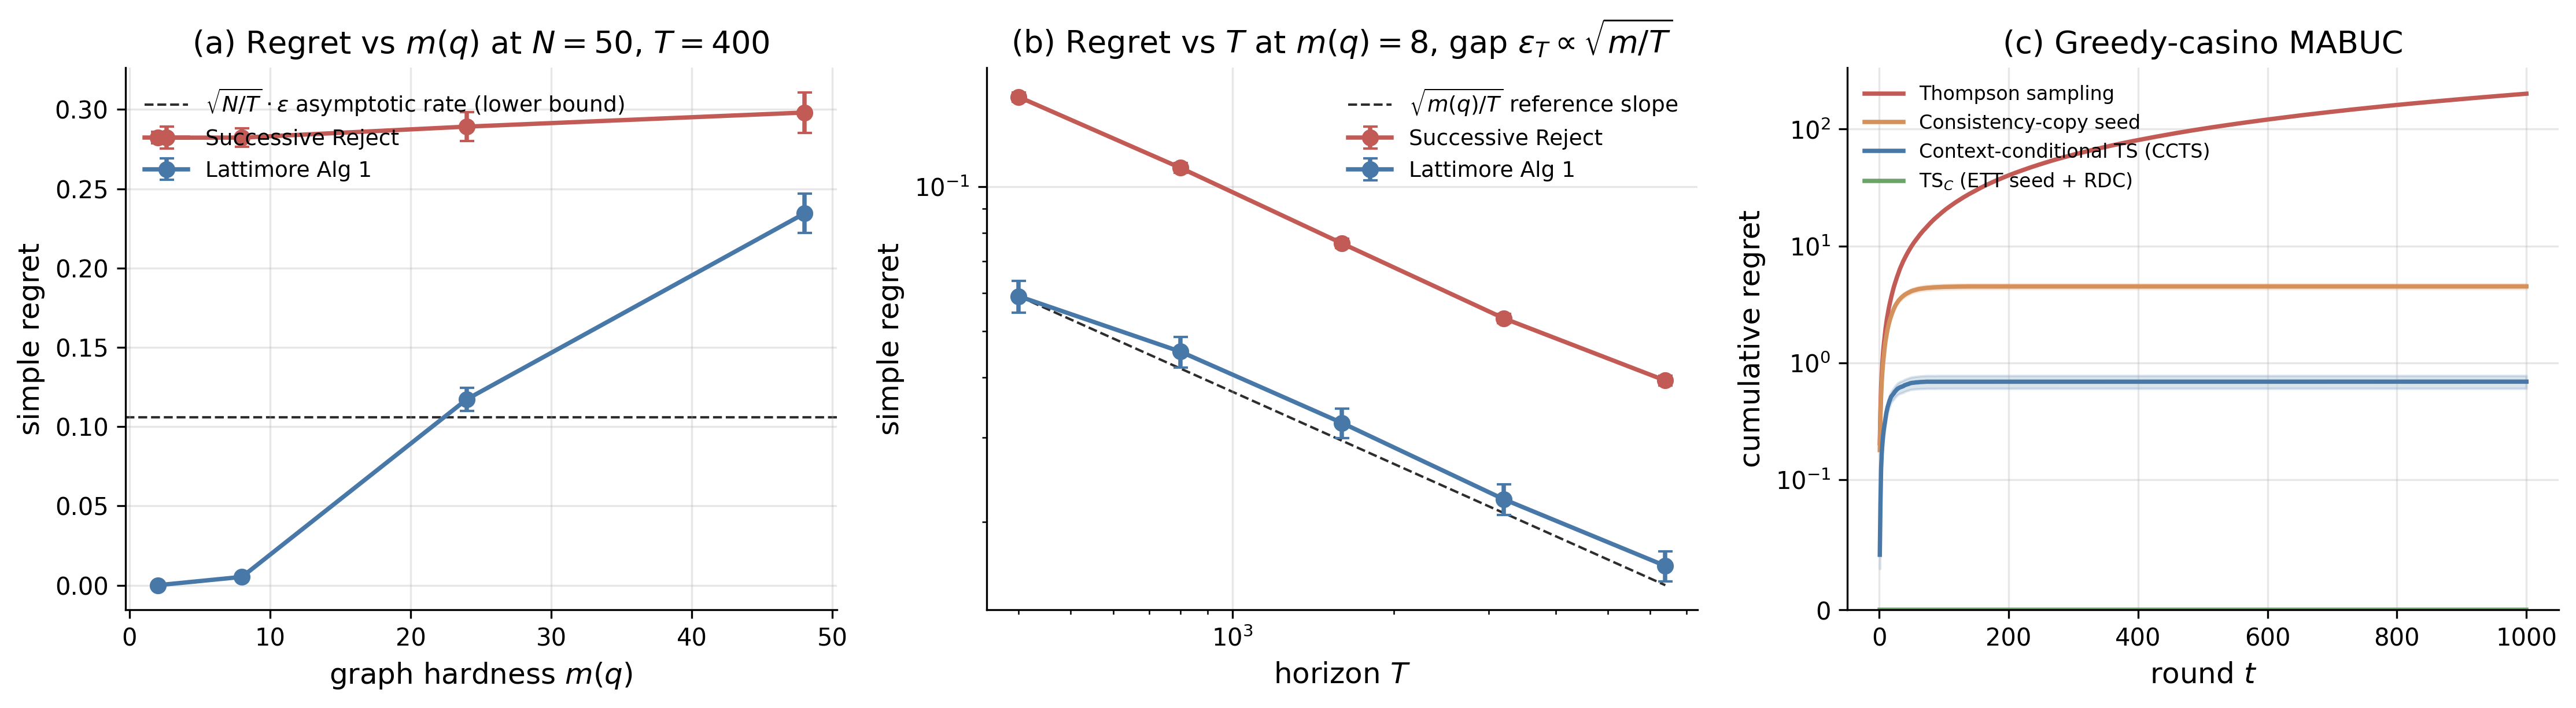
\includegraphics[width=\textwidth]{../ch10c_adaptive_experiments/sims/causal_bandit_combined.png}
\caption{Causal bandits. (a) Simple regret versus graph hardness $m(q)$ at fixed horizon $T = 400$, parent count $N = 50$ and gap $\epsilon = 0.3$; the dotted reference line is the $\sqrt{N/T} \cdot \epsilon$ lower bound on the asymptotic rate achievable by any graph-blind algorithm, not an upper bound on Successive Reject at finite $T$. (b) Simple regret versus horizon $T$ at fixed hardness $m(q) = 8$ with the gap shrinking as $\epsilon_T = \sqrt{m(q)/T}$, log-log axes; the dotted line is a $\sqrt{m(q)/T}$ reference slope anchored at the first cell, so only the slope is being compared. (c) MABUC greedy-casino panel under the unobserved-confounder instance of \citet[Table~1]{bareinboim2015mabuc}, on a symmetric-log vertical axis with a linear region below $0.1$ so that a curve at zero remains visible. The four traces span vanilla Thompson sampling, the consistency-copy seed, CCTS, and $\mathrm{TS}_C$. Error bars and shaded bands are 95\% confidence intervals. Replications are two thousand in (a), one thousand in (b) and five hundred in (c).}
\label{fig:simB2}
\end{figure}

All three claims survive, each on the panel built to test it. The ordering in $m(q)$ and the separation from a graph-blind baseline hold across the hardness grid, the $T^{-1/2}$ decay of \citet[Theorems~1--2]{lattimore2016causal} appears once the instance is held on the minimax frontier, and the counterfactual reasoning of \citet{bareinboim2015mabuc} converts a bandit problem with no marginal signal into one solved before the first round.

What the factorial adds is an attribution the aggregate comparison cannot give. Conditioning on intent is what makes the greedy casino tractable at all, and CCTS already does that, so the machinery specific to $\mathrm{TS}_C$ can only compete for the burn-in that conditioning alone leaves behind. On this instance it takes all of it. The lesson generalises past the example. The counterfactual seed is worth exactly the information the agent holds but cannot file, so its value scales with the interventional log and vanishes when the confounder is recorded; with two arms and two contexts the observational log's pessimism about one arm already implies the other, which bounds how much any refinement can win here and makes the instance a weak setting for measuring one.

%%%%%%%%%%%%%%%%%%%%%%%%%%%%%%%%%%%%%%%%%%%%%%%%%%%%%%%%%%%%%%%%%%%%%%%%%%%%%%%
\subsection{Discussion}
\label{subsec:adaptive_experiments_discussion}
%%%%%%%%%%%%%%%%%%%%%%%%%%%%%%%%%%%%%%%%%%%%%%%%%%%%%%%%%%%%%%%%%%%%%%%%%%%%%%%

Both sections of this chapter run the exchange between reinforcement learning and causal inference at the design stage rather than the estimation stage. The Lattimore causal bandit is the multi-armed bandit with the action set replaced by interventions on a known graph. The Kasy-Sautmann exploration sampling is Thompson sampling reshaped for a different objective function. The adaptively-weighted AIPW of \citet{hadad2021adaptive} is Robins-style augmented inverse-propensity weighting reweighted for adaptive data collection. In each case the move is not to invent a new algorithm but to recognize that an algorithm developed in one tradition addresses a question that arose in the other tradition.

Open problems remain in both directions. The matching minimax bound of \citet{lattimore2016causal} applies to the parallel-bandit setting; for general directed acyclic graphs the upper bound is established but the lower bound is not. The adaptively-weighted AIPW of \citet{hadad2021adaptive} assumes a known assignment mechanism; relaxing this to allow the analyst to recover valid inference from contextual bandit data collected by a black-box system is the contribution of \citet{bibaut2021post}, but the corresponding practical guidance remains to be developed. On the side of practice, the PAD India field experiment of \citet{kasy2021adaptive} is the chapter's clearest demonstration that the theory has practical purchase. A reinforcement-learning algorithm at the design stage, paired with a causal-inference estimator at the inference stage, produces valid welfare estimates on real participants in a real field setting, and the estimation machinery that consumes the resulting data is the subject of Chapter~\ref{section:rl_for_ci}.
